\justifying
\NSFCBodyText

% \subsubsection{研究内容}

% \subsubsubsection{职业发展轨迹纵向研究}
% 本研究以佐佐木希2002-2025年职业发展为案例，梳理职业路径，划分为五阶段（2002-2008时尚模特期、2008-2010转型期、2010-2017多领域拓展期、2017-2020成熟期、2020-2025重塑期），识别转型触发点。表\ref{tab:career_stages}展示了各阶段的核心特征与关键事件。

% \begin{table}[htbp]
%   \centering
%   \fontsize{11}{11}\selectfont
%   \caption{\textbf{佐佐木希职业发展五阶段特征对比}}
%   \begin{tabular}{lcccc}
%   \toprule
%   \textbf{阶段} & \textbf{时间跨度} & \textbf{核心领域} & \textbf{代表作品/事件} & \textbf{转型驱动力} \\
%   \midrule
%   时尚模特期 & 2002-2008 & 平面模特 & 《Pinky》《Non-no》 & 年龄增长 \\
%   转型期 & 2008-2010 & 影视试水 & 《热血街区》 & 职业拓展 \\
%   多领域拓展期 & 2010-2017 & 影视+综艺 & 多部电视剧 & 市场需求 \\
%   成熟期 & 2017-2020 & 全方位艺人 & 婚姻+事业 & 个人规划 \\
%   重塑期 & 2020-2025 & 新媒体转型 & YouTube频道 & 危机应对 \\
%   \bottomrule
%   \end{tabular}
%   \captionsetup{font={footnotesize,stretch=1.25},justification=raggedright}
%   \label{tab:career_stages}
% \end{table}

% \subsubsubsection{跨媒介形象构建机制}
% 分析不同媒介平台形象呈现策略，探讨“娃娃形象”的建构演变。

% \subsubsubsection{品牌韧性机制}
% 以2020年丈夫出轨风波为关键事件，分析个人品牌面临重大负面冲击时的应对策略。

% \subsubsubsection{新媒体转型策略}
% 研究从传统媒体向YouTube等新媒体平台的转型路径。

% \subsubsection{研究目标}

% \subsubsubsection{理论目标}
% 本项目总体目标是构建基于东亚文化语境的艺人职业发展动态分析框架。提出“艺人职业转型三阶段模型”（探索期-稳定期-重塑期），建立“跨媒介形象一致性测量指标体系”。

% \subsubsubsection{方法学目标}
% 开发“艺人职业轨迹编码手册”，构建“舆情事件影响评估模型”。

% \subsubsubsection{应用目标}
% 为娱乐产业从业者提供“艺人职业规划决策支持工具”。

% \subsubsection{拟解决的关键科学问题}

% \subsubsubsection{艺人职业转型的临界点识别问题}
% 如何科学识别关键转型节点？哪些内外部因素起决定性作用？

% \subsubsubsection{跨媒介形象的一致性维持问题}
% 如何在保持差异化形象的同时确保一致性？

% \subsubsubsection{个人品牌韧性的边界条件问题}
% 何种负面事件可通过特定策略修复？

% \subsubsection{研究方法}

% \subsubsubsection{纵向案例研究法}
% 本研究采用混合研究方法。收集完整职业档案（媒体报道约5000篇、影视作品约30部、商业代言约50个、社交媒体数据等），采用时序分析识别关键转折点。

% \subsubsubsection{内容分析法}
% 对时尚杂志约200期进行编码分析，提炼形象演变规律；对影视作品角色类型进行系统分类。编码工作由两名研究者独立完成，采用Cohen's Kappa系数评估信度（K>0.8）。

% \subsubsubsection{舆情分析法}
% 收集2020年出轨风波期间社交媒体舆情数据约10万条，运用情感分析和主题模型评估公众情绪变化。采用LDA模型进行主题分析，使用BERT预训练模型进行情感分类（准确率目标85\%以上）。

% \subsubsubsection{比较研究法}
% 选取同时期其他日本女性艺人（滨崎步、新垣结衣、石原里美等）作为对照案例，对比中日韩三国艺人发展模式异同。表\ref{tab:research_methods}总结了本研究采用的四种主要研究方法及其应用场景。

% \begin{table}[htbp]
%   \centering
%   \fontsize{11}{11}\selectfont
%   \caption{\textbf{研究方法体系与应用场景}}
%   \begin{tabular}{lccc}
%   \toprule
%   \textbf{研究方法} & \textbf{数据来源} & \textbf{分析工具} & \textbf{信度指标} \\
%   \midrule
%   纵向案例研究法 & 媒体报道5000篇 & 时序分析 & - \\
%   内容分析法 & 时尚杂志200期 & 编码分析 & Cohen's Kappa>0.8 \\
%   舆情分析法 & 社交媒体10万条 & BERT+LDA & 准确率>85\% \\
%   比较研究法 & 多案例对照 & 跨案例分析 & - \\
%   \bottomrule
%   \end{tabular}
%   \captionsetup{font={footnotesize,stretch=1.25},justification=raggedright}
%   \label{tab:research_methods}
% \end{table}

% 对于舆情情感分析，本研究采用基于BERT的情感分类模型，其情感得分计算公式为：
% \begin{equation}
% S(t) = \frac{1}{N} \sum_{i=1}^{N} w_i \cdot s_i(t)
% \label{eq:sentiment_score}
% \end{equation}
% 其中，$S(t)$表示时刻$t$的整体情感得分，$N$为样本数量，$w_i$为第$i$条评论的权重（基于转发量和点赞数），$s_i(t)$为第$i$条评论的情感极性得分（范围：-1到+1）。

% \subsubsection{技术路线}

% \subsubsubsection{数据收集与预处理}
% 本研究技术路线分四阶段（图\ref{fig:techroute}）。建立多源异构数据库，并将数据抓取、清洗、结构化存储与可追溯日志记录纳入同一流程。

% \lstinputlisting[
%   language=bash,
%   firstline=1,
%   lastline=14,
%   caption={数据处理流水线脚本示例（code/test.sh）},
%   label={code:data-pipeline}
% ]{code/test.sh}

% \subsubsubsection{职业轨迹建模}
% 应用序列分析识别职业发展典型路径，构建“职业状态转移矩阵”。

% \subsubsubsection{形象分析}
% 采用深度学习方法对影像资料进行特征提取，运用NLP技术分析文本资料。

% \subsubsubsection{模型验证与应用}
% 通过交叉验证和敏感性分析评估模型稳健性。

% \begin{figure}[htbp]
%   \centering
%   \includegraphics[width=0.85\textwidth]{figures/zzmx-115.jpg}
%   \caption{多阶段转型模型示意（projects/NSFC\_Young/figures/）。}
%   \label{fig:techroute}
% \end{figure}

% \begin{figure}[htbp]
%   \centering
%   \includegraphics[width=0.85\textwidth]{figures/zzmx-mobile-105.jpg}
%   \caption{移动端跨平台曝光与互动链路示意（projects/NSFC\_Young/figures/）。}
%   \label{fig:mobile-exposure}
% \end{figure}

% \subsubsection{关键技术}

% \subsubsubsection{多模态数据融合}
% 整合文本、图像、视频等多模态数据，构建统一知识图谱。

% \subsubsubsection{职业轨迹序列挖掘}
% 应用频繁序列模式挖掘算法识别职业发展典型模式。

% \subsubsubsection{舆情情感分析}
% 基于BERT、GPT等预训练模型进行日语文本情感分析（准确率85\%以上）。

% \subsubsection{可行性分析}

% \subsubsubsection{理论可行}
% 建立在成熟的职业发展理论、品牌管理理论、传播学理论基础之上。

% \subsubsubsection{数据可行}
% 佐佐木希公开资料丰富，Wikipedia、MyDramalist、AsianWiki等数据库提供充足数据源。

% \subsubsubsection{技术可行}
% 研究团队具备NLP、计算机视觉、数据挖掘技术储备。


%--------------------------------------------------------------------------
% 第一部分：研究内容主体现（总-分结构）
%--------------------------------------------------------------------------
% （15-18页，50\%-60\%,核心，展现完整设计
% 研究内容是标书核心，占15-18页，易出现"写长但讲不透"的问题。30页限制下需强化"用图说话"，提升图表权重，实现简洁高效表达。
% \textbf{该瘦的地方:}剔除冗余信息
% 重复表述:整合研究目标、内容、技术路线的重复内容，每个信息仅在最优位置出现一次，无需单独列段重复。
% 过细实验操作:标书非实验记录本，无需写清细节，仅保留核心思路与关键参数即可。
% 罗列式方法堆砌:避免"采用Western blot、qPCR等方法"的无意义罗列，需绑定具体研究问题，说明方法的应用目的与价值。
% 过度细化预期结果:无需大段描述预期结果，更不可提前"撰写"未做实验的数据，仅点明核心验证指标与判断标准。
% 冗长文字化步骤:用图表替代"第一步、第二步"的文字描述，文字仅作点睛之笔。
% \textbf{该厚的地方:}凸显研究核心价值研究内容的"厚"是核心逻辑与设计的深化，一张高质量图表的信息承载量堪比3页文字，重点厚在四方面:
% 研究递进逻辑:讲清从现象验证到机制探索、体外到体内、基础到转化的推进路径，展现清晰研究主线，避免内容碎片化。
% 关键实验设计:针对决定研究成败的1-2个关键实验，写透模型选择依据、分组逻辑、核心检测指标及结果验证假说的思路。
% 高质量可视化图表:重点打造科学机理图与技术路线交互图--技术路线图需涵盖步骤、关键参数、预期结果与风险预案;机理图清晰展现核心机制，直观传递创新性。
% 创新点实证论证:创新点不可喊口号，需用文献或前期数据支撑"首次发现"，用对比说明"新方法"优势，从理论、方法、应用维度证明创新价值。
% ）

\subsubsection{总体研究思路}

本项目以\textbf{``面向共身智能的高表现力社交动作感知、映射与生成机制研究''}为核心命题，遵循\textbf{``多维感知解耦（数据解析层） $\rightarrow$ 物理闭环映射（Sim-to-Real桥梁层） $\rightarrow$ 跨模态协同生成（认知-物理对齐层）''}的三层因果递进研究主线，针对轮盘式上半身人形机器人构型，建立从互联网人类社交视频出发、经物理约束桥梁、最终落地于真机高表现力交互的完整科学研究框架。本项目的总体研究内容与技术逻辑架构如图~\ref{fig:framework} 所示。

% 插入技术路线图占位符
\begin{figure}[!ht]
    \centering
    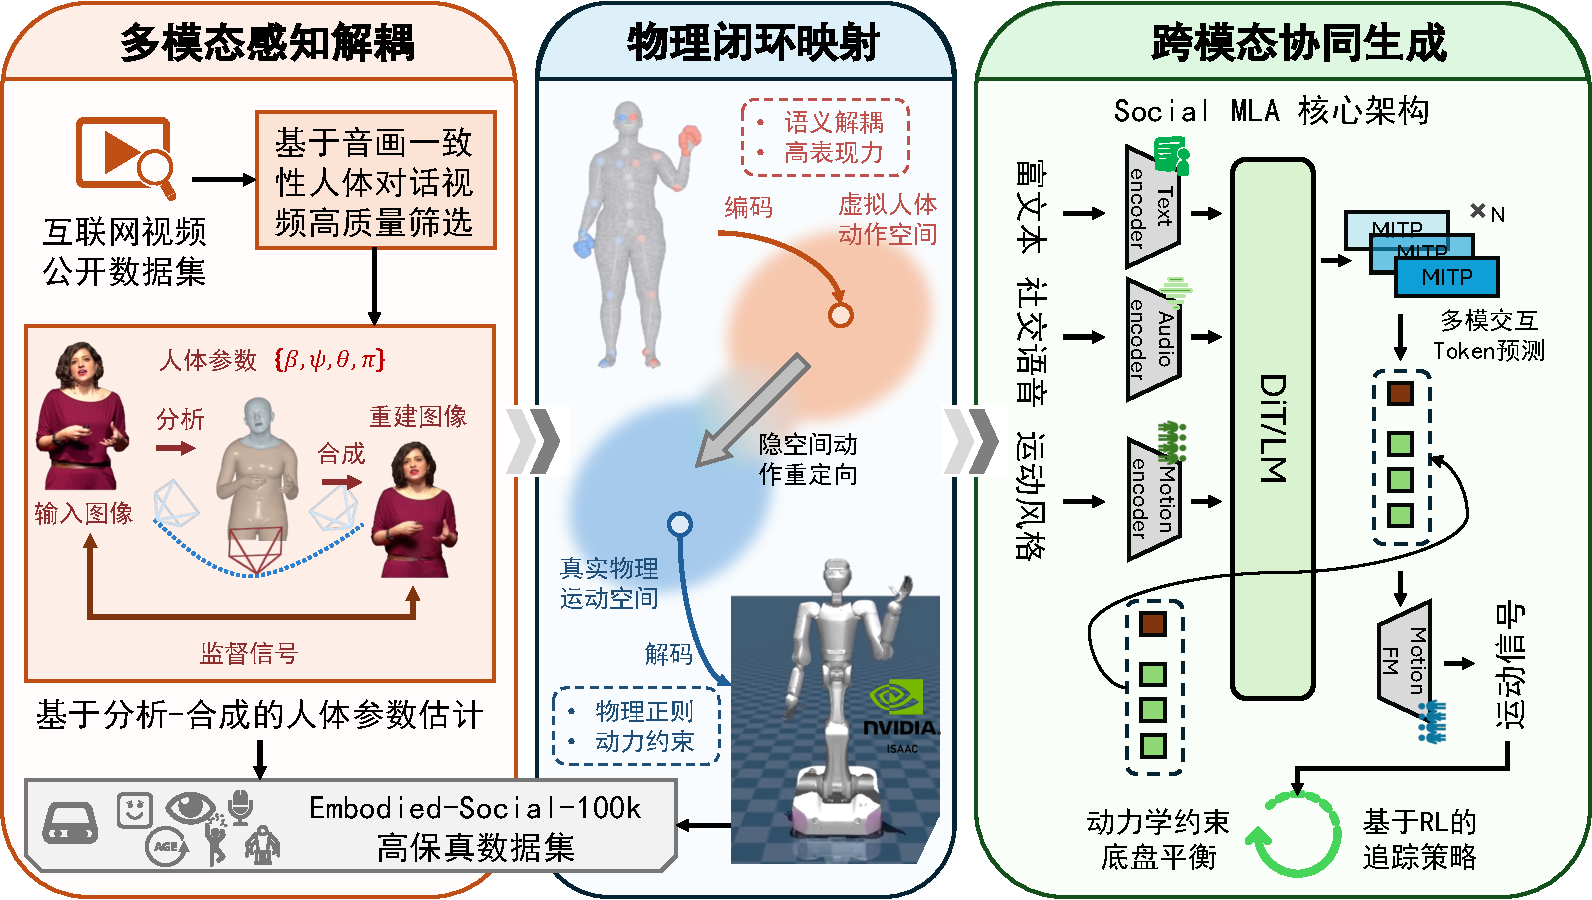
\includegraphics[width=\textwidth]{figures/framework.pdf} 
    \caption{\textbf{本项目研究内容与技术架构图。} 展示了本项目三层因果递进研究逻辑：（左）以Analysis-by-Synthesis联合估计框架解析``表情-视线-动作''多维耦合特征，构建\textbf{Embodied-Social-100k}高保真数据集；（中）以Isaac Lab物理引擎反馈闭环驱动异构动作重定向，建立运动学-动力学联合约束的非线性拓扑映射；（右）以\textbf{Social-MLA}（LM离散语义规划 + Flow Matching连续动作解码）实现跨模态动作流形的连续演化与对齐，最终在履带式人形机器人上实现高表现力社交交互。}
    \label{fig:framework}
\end{figure}

\textbf{第一层：数据解析层。}
以基于Analysis-by-Synthesis框架的联合估计机理为核心，攻克互联网视频数据和现有公开视频数据集中复杂交互遮挡下``表情-视线-动作''多维特征的时空同步解析难题；通过建立高精度的人体几何重建模型和高表现力人体参数模型，解耦情感判别性运动子空间与惯性运动子空间，为后续两层研究提供大量、多模态、语义感知先验。

\textbf{第二层：Sim-to-Real桥梁层。}
以Isaac Lab物理仿真引擎的动力学反馈为内生约束，突破传统静态IK重定向的局限，建立运动学-动力学联合约束的非线性拓扑映射优化框架；通过动力学边界补偿机制处理拓扑异构所导致的奇异性，探究虚拟人体动作分布到真实运动分布的隐空间映射，构建兼具情感保真性与物理安全性的共生社交数据集（Enbodied Social 100K）。

\textbf{第三层：认知-物理跨模态协同生成层。}在上述数据基础上，以\textbf{Social-MLA}（LM离散语义规划 + Flow Matching连续动作解码）为核心架构，探究情感语义离散表征对连续动作流形ODE演化的调制机理；以多部位时空耦合约束保障头-手-躯干协同生成的整体合理性；以轻量化RL追踪策略作为底层动力学安全辅助，最终在适老化陪护场景中验证Social-MLA的综合交互效能。


\subsubsection{具体研究内容与实施方案}

\subsubsubsection{研究内容一：复杂交互语境下的多模态感知解耦与参数化重构}

正如本项目科学问题一所述，当前具身智能领域生成大模型（如VLA框架）面临的情感表现力缺失，其根源在于上游训练数据的贫瘠。传统的遥操作（Teleoperation）数据不包含面部与社会化手势，而现有的互联网动作捕捉技术（Motion Capture in-the-wild）往往孤立地处理人体的各个部位，缺乏对“表情-视线-动作”在复杂社交交互场景下的强时空耦合关联建模。

为此，本项目如图~\ref{fig:framework}左侧“多模态感知解耦”模块所示，拟建立从海量非结构化互联网视频与公开数据集中，逆向重构高精度虚拟人体动作空间（Virtual Human Motion Space）的全栈数据解析管线。本研究内容将重点突破基于音画一致性的高价值数据挖掘、遮挡环境下的多维特征时空同步解析，以及基于“分析-合成（Analysis-by-Synthesis）”的闭环参数化估计等关键技术，为下游的Sim-to-Real物理闭环映射提供语义解耦且高保真的感知先验。本模块具体包含以下三个递进的研究线索：

\paragraph{\textbf{研究线索 1.1：基于音画一致性的高价值社交交互视频精细化筛选与多模态对齐机理}}

高质量的具身生成基座模型严重依赖于规模化且语义严格对齐的数据支撑。尽管互联网中存在海量的对话、演讲、访谈等人类社交视频（如图~\ref{fig:framework}左上角所示的输入端），但此类公开原始数据普遍存在音画不同步、背景噪声干扰、多说话人重叠（Cocktail Party Effect）以及由于镜头频繁切换导致的动作时序割裂等“脏数据”问题。若直接将此类异构数据馈入3D位姿估计网络，将导致模型不可避免地学习到错误的“语义-动作”因果映射（Spurious Correlations）。因此，建立一套严密的、基于跨模态物理约束的高效过滤与筛选机制，是构建 Embodied-Social-100k 数据集的先决条件。

本项目拟重点探究多模态信号在时域与频域空间中的强相关性判别模型。首先，针对视频帧序列 $\mathcal{V} \in \mathbb{R}^{T \times H \times W \times 3}$ 与对应的原始一维音频信号 $\mathcal{A} \in \mathbb{R}^{T'}$，引入具备高时序分辨率的主动说话人检测（Active Speaker Detection, ASD）与音画同步关联网络。具体实现上，采用双流特征编码架构：视觉流利用时空三维卷积（如3D-ResNet）提取说话人面部（特别是唇部与下颌运动）的细粒度视觉动态特征序列 $\mathbf{f}_{v} \in \mathbb{R}^{T \times d}$；音频流则通过短时傅里叶变换（STFT）提取Mel频谱图，并经由1D-CNN编码为音频特征序列 $\mathbf{f}_{a} \in \mathbb{R}^{T \times d}$。
为精确量化两者的同步状态，构建跨模态对比学习损失（Cross-modal Contrastive Loss），通过计算 $\mathbf{f}_{v}$ 与 $\mathbf{f}_{a}$ 之间的余弦相似度轨迹，提取音画同步置信度标量 $S_{sync}(t)$。结合心理声学模型中人耳对音画不同步的感知阈值（通常为视觉超前 45ms 或滞后 125ms），设定自适应的软阈值边界，精确截取严格对齐的视频片段，从源头上剔除由后期配音或网络延迟造成的错位样本。

进一步地，针对具身智能交互场景对“非语言行为表达”的特殊需求，设计面向高表现力（High-Expressivity）特征的片段价值挖掘算法。由于大量日常对话视频中人物躯干处于静止状态，缺乏丰富的伴随手势（Co-speech Gestures），此类低熵数据对训练模型的泛化能力贡献极其有限。本项目拟提出一种“运动表现力熵（Motion Expressivity Entropy）”的量化评价指标。通过轻量级2D人体关键点检测器提取画面中说话人的骨架关键点坐标序列 $\mathbf{K}_{2D}(t)$，计算其腕关节速度分布的方差、手部运动轨迹的凸包面积（Convex Hull Area）以及面部关键点（如眉毛、嘴角）的激活频次。综合多维度的运动学统计特征，赋予每个视频片段一个表现力得分 $S_{expr}$。最终，构建融合 $S_{sync}$ 与 $S_{expr}$ 的联合排序算法，实现对海量互联网视频的自动化、高质量、无人工干预的“沙里淘金”，确保输送至下一阶段的切片不仅语义对齐，且富含高频互动的社交动作模式。

\paragraph{\textbf{研究线索 1.2：复杂交互与自遮挡条件下的多维特征时空同步解析架构}}

在获取高质量视频切片后，提取其中的三维人体运动学参数是构建虚拟人体动作空间的核心。然而，真实的面对面社交交互不可避免地存在严重的肢体自遮挡（如手部托腮、双手交叉）以及人与环境/他人的互遮挡。传统的基于单帧图像直接回归（Direct Regression）的人体网格恢复算法，由于将头部、手部与躯干视作相互独立的感受野（Receptive Fields）进行处理，在遭遇局部遮挡时极易产生不可逆的姿态坍塌（Pose Collapse）或深度模糊（Depth Ambiguity）。

为打破这一局限，本项目提出构建基于联合注意力机制的时空同步解析网络。该网络旨在挖掘人类非语言行为中“牵一发而动全身”的时空耦合先验（如：情绪高昂时，视线聚焦、眉毛上扬与手势的顶点在时间轴上往往呈现毫秒级的共现）。网络以前馈方式处理输入的RGB视频片段，提取全局与局部特征。
在空域维度，摒弃传统将人体强行裁剪为多个独立Patch的割裂做法，引入具有全局感受野的Vision Transformer (ViT) 作为骨干网络。通过在网络深层设计显式的拓扑注意力掩码（Topology-aware Attention Mask），使得被严重遮挡的末端关节（如被身体遮挡的手掌）的特征重建，能够强依赖于其父节点（如手肘、肩膀）的运动状态以及面部表情的语义提示。在时域维度，引入时序卷积网络（TCN）与门控循环单元（GRU）的混合架构，在潜变量空间（Latent Space）中强制执行低通滤波平滑约束，利用前后帧的运动学连续性来补偿单帧中缺失的视觉观测信息，从而在隐空间层面实现高维特征矩阵的初步去噪与结构化解耦。

\paragraph{\textbf{研究线索 1.3：基于“分析-合成（Analysis-by-Synthesis）”的闭环参数化重构与监督信号设计}}

前馈神经网络虽能快速预测人体姿态的粗略分布，但在面部微表情、视线方向（Gaze）与手指精细动作等细粒度高频特征的拟合上依然存在不可忽视的误差。为获取足以支撑高表现力具身控制的“专家级”运动轨迹，本项目如图~\ref{fig:framework}左下方核心虚线框所示，提出建立基于“分析-合成（Analysis-by-Synthesis）”范式的可微闭环优化模型。

首先，统一参数化表达体系。采用SMPL-X（SMPL eXpressive）作为核心人体模型，其拓扑结构可由一组紧凑的参数集合 $\Phi = \{\beta, \psi, \theta, \pi\}$ 唯一确定。其中，$\beta \in \mathbb{R}^{10}$ 表征人体的身份与体型形状参数（Shape）；$\psi \in \mathbb{R}^{50}$ 为由面部动作编码系统（FACS）驱动的表情基系数（Expression），负责刻画微笑、蹙眉等瞬态情感特征；$\theta \in \mathbb{R}^{(J+2) \times 3}$ 囊括了包含脊柱、颈部与高自由度灵巧手指在内的全身相对旋转姿态（Pose）；$\pi$ 表征全局根节点的平移矩阵与弱透视相机的投影参数。

\textbf{分析与合成过程的数学建模：}
在每一次优化迭代中，“合成（Synthesis）”阶段将当前网络预测的参数 $\hat{\Phi}$ 馈入可微的三维人体网格回归器。根据前向运动学（Forward Kinematics, FK）计算出 $N=10475$ 个顶点的三维空间坐标 $\mathbf{V} \in \mathbb{R}^{N \times 3}$，并利用线性混合蒙皮（Linear Blend Skinning, LBS）算法处理网格变形。随后，通过可微渲染器（Differentiable Renderer） $\mathcal{R}(\cdot)$，将带有纹理的人体三维网格 $\mathbf{V}$ 投影回二维像平面，生成重建的虚拟图像 $\mathcal{I}_{recon} = \mathcal{R}(\mathbf{V}(\hat{\Phi}), \hat{\pi})$。

在此基础上，设计极为严密的闭环“监督信号（Supervision Signals）”，构建驱动参数 $\hat{\Phi}$ 逼近真实物理运动流形的联合能量目标函数 $E_{total}(\Phi)$。该目标函数由数据项与先验约束项复合而成：
\begin{equation}
\label{eq:optimization}
E_{total}(\Phi) = \lambda_{photo}\mathcal{L}_{photo} + \lambda_{kp}\mathcal{L}_{kp} + \lambda_{prior}\mathcal{L}_{prior} + \lambda_{temp}\mathcal{L}_{temp}
\end{equation}

1) \textbf{光度一致性约束 ($\mathcal{L}_{photo}$)}：直接计算输入原图 $\mathcal{I}_{in}$ 与重建图像 $\mathcal{I}_{recon}$ 在面部及手部高频纹理区域的像素级L1范数差异。该项强迫模型精准捕获由面部肌肉群牵引导致的皮肤褶皱变化，是提取微小情感语义特征的关键。
2) \textbf{运动学投影误差 ($\mathcal{L}_{kp}$)}：计算三维关节坐标重投影后与现成2D关键点检测器提取的坐标（如OpenPose）的加权鲁棒Huber损失，确保整体骨架的空间位置不发生宏观漂移。
3) \textbf{混合高斯姿态先验 ($\mathcal{L}_{prior}$)}：由于从2D到3D的逆向映射属于典型的病态问题（Ill-posed Problem），存在多解性。本项目引入预训练的VPoser变分自编码器构建姿态空间先验，对产生非自然人体骨架扭曲（如关节角度超出人体生理极限）的参数 $\hat{\theta}$ 施加指数级惩罚。
4) \textbf{高阶时序平滑正则化 ($\mathcal{L}_{temp}$)}：为满足机器人底盘控制对指令平滑性的极高要求，在目标函数中对相邻帧的参数引入一阶速度与二阶加速度的二阶差分惩罚：$\mathcal{L}_{temp} = \sum_{t} \|\hat{\Phi}_t - 2\hat{\Phi}_{t-1} + \hat{\Phi}_{t-2}\|^2_2$。该设计从源头消除了高频抖动噪声，确保重构数据的物理可用性。

经过上述基于Analysis-by-Synthesis的交替下降与非线性优化求解，系统能够将二维视频像素空间中纠缠的光度、几何与时间信息，深度解耦为具有物理与语义双重属性的纯净三维人体参数序列。这批数据将作为极高质量的“虚拟人体动作分布”，无缝输送至本项目的第二层（中框）研究中，接受Isaac Lab物理引擎的动力学闭环映射与严苛筛选。

% ============================================================================

\subsubsubsection{研究内容二：受限物理实体约束下的隐空间闭环映射与数据集构筑}

通过研究内容一的“分析-合成”管线，本项目已从海量互联网视频中解耦并提取出高精度的三维人体参数序列。然而，如图~\ref{fig:framework} 中间的“物理闭环映射”模块所示，从“虚拟人体动作空间（Virtual Human Motion Space）”到“真实物理运动空间（Real Physical Motion Space）”的跨越，面临着不可逾越的拓扑异构性（Topological Heterogeneity）与动力学鸿沟（Dynamics Gap）。高达145个自由度的柔性人体骨架与极度受限的刚性机器人（约20-30个自由度）之间，不仅存在一对多的病态映射关系，且由于人体数据完全脱离了机器人自重、电机力矩极限与履带底盘的摩擦约束，直接应用传统运动学解算将导致严重的物理违例与动作语义折损。

为此，本模块旨在突破传统静态逆运动学（IK）的理论局限，探究融合语义先验的隐空间动作重定向（Latent Space Motion Retargeting）机理，并将Isaac Lab物理引擎的动力学反馈作为内生约束引入优化闭环，最终构筑兼具高表现力与物理安全性的 Embodied-Social-100k 数据集。具体包含以下三个递进的研究线索：

\paragraph{\textbf{研究线索 2.1：基于拓扑异构的隐空间动作重定向与语义解耦机理}}

传统的重定向方法多在原始的三维关节欧氏空间（Euclidean Space）中通过最小化关节点距离（如MSE）来求解。这种生硬的几何映射会强制裁剪掉机器人无法复现的微小自由度，从而系统性地抹除诸如“轻微耸肩”、“手腕翻转”等承载高表现力的关键社交特征。本项目提出摒弃欧氏空间的直接映射，转而在高维流形的隐空间（Latent Space）中寻求跨实体的运动学对齐。

首先，构建面向虚拟人体动作空间与真实物理运动空间的非对称自编码器（Asymmetric Autoencoder）架构。定义源域为人体动作特征序列 $\mathbf{X}_H \in \mathbb{R}^{T \times D_H}$，目标域为机器人关节角度序列 $\mathbf{X}_R \in \mathbb{R}^{T \times D_R}$。设计深层时空图卷积网络（ST-GCN）作为编码器 $\mathcal{E}_H(\cdot)$，将异构的人体运动学链映射至一个共享的低维隐空间 $\mathcal{Z} \in \mathbb{R}^{T \times d_z}$，即 $\mathbf{z} = \mathcal{E}_H(\mathbf{X}_H)$。
为实现图~\ref{fig:framework}中所标示的“语义解耦（Semantic Decoupling）”与“高表现力（High Expressivity）”保留，本项目在隐空间 $\mathcal{Z}$ 中引入对比学习（Contrastive Learning）与正交子空间投影机制。具体而言，将隐编码 $\mathbf{z}$ 显式解耦为情感语义特征 $\mathbf{z}_{sem}$ 与结构姿态特征 $\mathbf{z}_{pose}$。通过构建社交动作原语词典（Social Action Primitives Dictionary），对具有相同社交意图（如“安抚”、“拒绝”）但姿态略有不同的运动序列施加正样本拉近约束，强制 $\mathbf{z}_{sem}$ 捕获独立于本体拓扑结构的纯粹情感动态特征。

随后，设计适配于目标机器人运动学树（Kinematic Tree）的解码器 $\mathcal{D}_R(\cdot)$。解码过程并非简单的全连接映射，而是采用自回归的循环神经网络结构，将解耦后的隐变量解码为机器人关节序列：$\hat{\mathbf{X}}_R = \mathcal{D}_R(\mathbf{z}_{sem}, \mathbf{z}_{pose})$。在此阶段，定义运动学重定向损失函数 $\mathcal{L}_{retarget}$：
\begin{equation}
\mathcal{L}_{retarget} = \alpha_1 \|\mathbf{X}_H^{EE} - \mathcal{F}_{fk}(\hat{\mathbf{X}}_R)^{EE}\|^2_2 + \alpha_2 \mathcal{L}_{velocity} + \alpha_3 \mathcal{L}_{self-collision}
\end{equation}
其中，第一项约束了源实体与目标实体在关键末端效应器（End-effector，如手掌心、头部朝向）在标准化空间中的相对轨迹一致性（即空间保真度）；$\mathcal{F}_{fk}(\cdot)$ 为机器人前向运动学求解函数；$\mathcal{L}_{velocity}$ 确保动作节律（如挥手的频率）的严格同步；$\mathcal{L}_{self-collision}$ 则是基于距离场（SDF）的自碰撞惩罚项，用于避免双臂在胸前交叉时发生物理干涉。

\paragraph{\textbf{研究线索 2.2：基于Isaac Lab物理引擎的闭环映射与动力学正则化机制}}

仅依赖隐空间的运动学映射，虽然能够保证动作的语义高保真度，但在物理世界中往往是极其危险且不可执行的。例如，人体在激烈演讲时重心的快速偏移，若直接映射至履带式人形机器人，极易超出其零力矩点（ZMP）的稳定多边形，导致倾覆。因此，必须将“物理闭环（Physical Closed-loop）”引入映射过程。

本项目如图~\ref{fig:framework}中框的下半部分所示，创新性地将NVIDIA Isaac Lab高保真物理仿真引擎封装为一个可微分（或通过强化学习进行梯度估计）的物理层 $\mathcal{P}_{sim}(\cdot)$。将解码器输出的运动学轨迹 $\hat{\mathbf{X}}_R$ 作为参考轨迹，输入至Isaac Lab中进行正向动力学仿真。在仿真环境中，机器人不仅受到刚体动力学（Rigid Body Dynamics）的约束，还受到履带与地面摩擦力、关节伺服电机峰值力矩以及重力加速度的综合作用。
仿真引擎将输出执行该轨迹时的真实物理状态序列 $\mathbf{S}_{sim} = \{\mathbf{q}, \dot{\mathbf{q}}, \mathbf{\tau}, \mathbf{c}_{com}\}$（分别代表关节位置、速度、控制力矩及全局质心坐标）。基于此反馈，本项目构建严苛的“物理正则化（Physical Regularization）”与“动力约束（Kinematic Constraints）”惩罚函数 $\mathcal{L}_{physics}$：
\begin{equation}
\mathcal{L}_{physics} = \lambda_{\tau} \sum_{t} \max(0, \|\mathbf{\tau}_t\| - \mathbf{\tau}_{max}) + \lambda_{com} \sum_{t} \mathcal{D}(\mathbf{c}_{com}(t), \mathcal{P}_{support}) + \lambda_{jerk} \sum_{t} \|\dddot{\mathbf{q}}_t\|^2_2
\end{equation}
上式中，第一项为电机力矩超限惩罚，强制剥离那些导致关节过载的高频剧烈动作；第二项为质心偏移惩罚，$\mathcal{D}(\cdot)$ 计算实时质心 $\mathbf{c}_{com}$ 到履带底盘支撑多边形 $\mathcal{P}_{support}$ 边界的距离，确保在大幅度社交动作中底盘的绝对平衡；第三项为加加速度（Jerk）惩罚，保证动作的平滑度以延长机械臂寿命。

关键的创新点在于：本项目将上述物理正则项 $\mathcal{L}_{physics}$ 作为梯度反馈信号（Gradient Feedback Signal），反向传播至隐空间的解码器 $\mathcal{D}_R(\cdot)$ 与编码器 $\mathcal{E}_H(\cdot)$ 中。通过“隐空间运动学重构”与“物理引擎动力学校验”的端到端联合优化，网络能够自动学会一种**动力学边界补偿机制**——当某一人体社交动作（如深度鞠躬）在机器人上不可行时，网络不再生硬地截断动作，而是学会在隐空间中通过微调其他代偿关节（如微屈手臂、后移底盘）来维持相同的“社交语义特征”，从而实现表现力与安全性的联合最优解。

\paragraph{\textbf{研究线索 2.3：高保真 Embodied-Social-100k 数据集的并行化构筑}}

基于上述运动学-动力学联合约束的非线性拓扑映射框架，本项目将启动大规模数据的自动化清洗与构筑流水线。利用Isaac Lab强大的GPU并行张量加速能力（Tensor-based Simulation API），在仿真空间中同时实例化数千个带有不同社交动作参考轨迹的机器人环境（Envs）。

针对筛选后的人类互联网交互视频，系统性地执行“感知解耦 $\rightarrow$ 隐空间映射 $\rightarrow$ 物理引擎闭环校验 $\rightarrow$ 动态重优化”的完整流转。只有那些在Isaac Lab中能够稳定执行、未触发任何碰撞阈值、且电机能耗收敛于正常区间内的轨迹序列，才会被系统最终验收。
验收通过的数据将被打包整合，正式定型为图~\ref{fig:framework}左下方标注的 \textbf{Embodied-Social-100k 高保真数据集}。该数据集将首次在国际上提供包含“富文本指令-人类社交音频-隐空间动作Token-物理安全的机器人URDF运动轨迹-底层力矩曲线”的多模态严格对齐样本。这一独有的数据资产，彻底填补了图形学虚拟生成与机器人底层控制之间的数据鸿沟，为后续第三层（右框）跨模态协同生成大模型（Social MLA）的训练，提供了不可或缺、且兼具“情感高表现力”与“真机直接可部署性”的硬核数据支撑。

% ===========================================

\subsubsubsection{研究内容三：Social MLA 核心架构驱动的跨模态协同生成与虚实迁移}

依托前述研究内容构筑的 Embodied-Social-100k 高保真物理数据集，本项目已彻底打通从多模态感知到物理安全运动状态的底层映射流转。然而，如图~\ref{fig:framework} 右侧“跨模态协同生成”模块所示，面对未知的社交场景指令，如何使得机器人实时、自发地生成兼具情感表现力与动力学平滑性的连续交互动作，仍面临着“离散语义表征”与“连续物理流形”跨模态对齐的根本性理论鸿沟。

为此，本项目提出并构建面向共身智能的 \textbf{Social MLA（Social Multi-modal Large Architecture）核心架构}。该架构突破了传统端到端回归模型的时序模糊性局限，创新性地采用“大语言模型（LM）离散语义规划 + 流匹配（Flow Matching）连续动作解码”的级联演化范式。本模块将重点探究多模态Token的交互预测机理、连续具身动作流形的ODE演化规律，以及基于强化学习的底盘平衡控制，最终实现高表现力动作在真实物理世界的高保真部署。具体包含以下三个递进的研究线索：

\paragraph{\textbf{研究线索 3.1：离散语义驱动的多模态交互Token预测（MITP）与DiT/LM特征融合机理}}

高表现力的社交交互行为（如：伴随惊讶语气的后仰与手势停顿）在本质上具有高度的“组合性（Compositionality）”与语义结构化特征。传统的扩散模型（Diffusion Models）往往在连续像素或运动学空间直接加噪去噪，难以显式地建模高层的情感逻辑关联。因此，Social MLA架构的首要任务是在高维隐空间中构建多模态语义的对齐与离散化表征机制。

如图~\ref{fig:framework}右侧上半部所示，首先构建异构多通道编码器（Heterogeneous Encoders）。针对输入的\textbf{富文本（Text）}指令集 $\mathcal{T}$，采用预训练的语言模型（如RoBERTa）提取深层意图特征 $\mathbf{h}_{text}$；针对输入的\textbf{社交语音（Audio）}片段 $\mathcal{A}$，引入Wav2Vec 2.0架构提取蕴含情感与节奏的声学副语言特征（Paralinguistic Features） $\mathbf{h}_{audio}$；同时，针对特定的\textbf{运动风格（Motion Style）}条件提示 $\mathcal{S}$，设计风格特征编码器提取风格潜向量 $\mathbf{h}_{style}$。
为解决跨模态特征在时空维度的异构性，本项目引入基于 \textbf{DiT/LM（Diffusion Transformer / Language Model）} 的混合骨干网络。将上述多模态特征投影至统一维度的隐空间，并通过多头交叉注意力机制（Cross-Attention）实现声学韵律与文本语义在时间步上的精准对齐。

在此基础上，提出\textbf{多模交互Token预测（Multi-modal Interactive Token Prediction, MITP）}机制。我们将连续的具身动作序列通过预训练的神经离散表示向量量化器（如VQ-VAE的Codebook）离散化为有限的“社交动作词表（Social Action Vocabulary）”。利用大语言模型（LM）强大的自回归（Auto-regressive）上下文推断能力，将多模态融合特征作为前缀提示（Prompt），在时间轴上自回归地预测出长度为 $N$ 的离散语义Token序列 $\hat{Z} = \{z_1, z_2, \dots, z_N\}$。
这一机制的核心机理在于：通过离散Token的规划，LM网络能够在宏观语义层面对诸如“点头”、“摊手”、“躯干前倾”等基础社交动作原语（Primitives）进行时序上的逻辑编排，从而确保机器人生成的长时序动作序列在社交语境下具备高度的情感一致性与语义合理性，为后续的连续运动解码提供了严格的“离散语义骨架”。

\paragraph{\textbf{研究线索 3.2：基于流匹配（Flow Matching）的连续具身动作流形解码与演化机理}}

尽管MITP机制成功输出了富含情感逻辑的离散Token序列 $\hat{Z}$，但物理机器人的底盘电机与双臂关节执行器需要的是具备二阶连续可导属性的连续控制信号（即位置、速度指令）。若直接对离散Token进行最近邻解码插值，将引发严重的关节高频抖动（Jittering），进而损坏减速器或诱发底盘共振。

针对这一跨模态鸿沟，本项目如图~\ref{fig:framework}右侧核心流线所示，创新性地引入\textbf{流匹配（Motion Flow Matching, FM）}作为连续动作解码器。相比于传统扩散模型中离散时间步的马尔可夫链加噪，流匹配通过构建连续时间的常微分方程（ODE），直接在目标运动数据分布与先验噪声分布之间构造最优传输（Optimal Transport）的确定性向量场，具有更优的轨迹平滑性与极高的采样效率。
具体而言，设真实的连续机器人运动轨迹数据服从分布 $q(\mathbf{x})$，定义一个从标准正态分布 $p_0(\mathbf{x}) = \mathcal{N}(0, I)$ 到目标数据分布 $p_1(\mathbf{x}) \approx q(\mathbf{x})$ 的连续概率密度路径 $p_t(\mathbf{x})$（其中时间标量 $t \in[0, 1]$）。流匹配的核心在于学习一个由神经网络参数化的时变向量场 $v_\theta(\mathbf{x}_t, t, c)$，使其逼近边缘向量场 $u_t(\mathbf{x}_t)$。
本项目将DiT（Diffusion Transformer）作为底层架构对 $v_\theta$ 进行参数化，并引入由线索3.1输出的离散交互Token $\hat{Z}$ 以及音频融合特征作为强条件引导（Conditioning $c$）。目标损失函数 $\mathcal{L}_{FM}$ 形式化为：
\begin{equation}
\mathcal{L}_{FM}(\theta) = \mathbb{E}_{t \sim \mathcal{U}[0,1], \mathbf{x}_1 \sim q, \mathbf{x}_0 \sim p_0} \left[ \left\| v_\theta(\mathbf{x}_t, t, \hat{Z}) - (\mathbf{x}_1 - \mathbf{x}_0) \right\|^2_2 \right]
\end{equation}
在推理（Inference）阶段，模型只需从高斯白噪声 $\mathbf{x}_0$ 出发，在离散语义Token $\hat{Z}$ 的条件引导下，使用如Euler法等数值积分器求解常微分方程 $d\mathbf{x}_t = v_\theta(\mathbf{x}_t, t, \hat{Z}) dt$，积分至 $t=1$ 即可确定性地生成连续的\textbf{运动信号（Motion Signals）}。
这一机制从根本上揭示了\textbf{跨模态协同生成的理论本质}：即以离散的社交意图Token $\hat{Z}$ 调制常微分方程的非线性漂移项，迫使生成的连续物理运动流形严格沿着人类社交情感的概率边界演化，从而彻底打破了图形学数字人生成“平滑却无逻辑”与自回归模型“有逻辑却不连续”的工程僵局。

\paragraph{\textbf{研究线索 3.3：融合底盘平衡与动力学约束的强化学习追踪策略与虚实迁移真机验证}}

依托Social MLA架构，系统已能输出兼具情感语义与时序平滑性的参考轨迹（Reference Trajectories）。然而，真实的履带式人形机器人在执行高表现力交互动作时，上半身（双臂与重型躯干）的大幅挥动与瞬态前倾会产生极大的动态扰动力矩。若仅依赖底层电机的传统位置伺服（PD Control），极易引发履带底盘的打滑、抬起甚至整体倾覆。

为此，如图~\ref{fig:framework}右下角所示，本项目提出构建\textbf{基于强化学习（RL）的鲁棒追踪策略}，完成从仿真空间向真实物理世界的“最后一公里”闭环迁移（Sim-to-Real Deployment）。
在Isaac Lab / MuJoCo 仿真环境中，将底盘与上半身作为一个耦合的多刚体动力学系统进行建模。定义RL策略网络 $\pi_\phi(\mathbf{a}_t | \mathbf{s}_t)$，其状态空间 $\mathbf{s}_t$ 不仅包含机器人的本体感知数据（关节角度、角速度、IMU测量的底盘俯仰/横滚角），还通过观测历史窗口融合了由Social MLA生成的未来参考轨迹帧 $\mathbf{x}_{ref}(t:t+H)$。动作空间 $\mathbf{a}_t$ 输出为各伺服电机的目标位移或前馈力矩指令。
针对高动态社交交互对底盘稳定性的严苛要求，本项目设计深度耦合的复合奖励函数（Reward Function） $\mathcal{R}_t$：
\begin{equation}
\mathcal{R}_t = \omega_{trk} \exp(-\|\mathbf{q}_t - \mathbf{q}^{ref}_t\|^2_2) + \omega_{bal} \exp(-\| \dot{\mathbf{r}}_{chassis} \|^2_2) - \omega_{\tau} \|\mathbf{\tau}_t\|_2^2 - \omega_{cmd} \|\mathbf{a}_t - \mathbf{a}_{t-1}\|_2^2
\end{equation}
其中，第一项驱动机器人对Social MLA输出的高表现力动作进行高精度几何追踪；第二项 $\omega_{bal}$ 为关键的\textbf{底盘平衡约束（Chassis Balance Constraints）}，严厉惩罚履带底盘在俯仰（Pitch）与横滚（Roll）方向的非预期角速度 $\dot{\mathbf{r}}_{chassis}$，迫使策略网络学会在上半身剧烈运动时，通过微调履带电机的差速补偿来抵消质心偏移；后两项则限制了能量消耗与控制指令的高频突变（Jerk），实现\textbf{功耗均衡}与动作柔顺。

最终，通过Domain Randomization（域随机化，包括扰乱质量分布、履带摩擦系数与电机响应延迟）提升RL策略的鲁棒性。将训练收敛的追踪策略零样本（Zero-shot）部署至真实的履带式人形机器人上。在面向适老化陪护、自然语音问答等典型人机共融场景中，系统性验证机器人在物理世界中执行诸如“附和点头”、“摊手安慰”、“激动演讲”等高表现力动作的自然度、安全性与底盘抗扰动能力，全面验证Social MLA核心架构的科学合理性与落地可行性。

